\subsection{1.1 Unit conversions}
	\begin{itemize}
  		\item \textbf{Energy:} $1eV=1.602\cdot 10^{-19}J$,    $1cal=4.18J$
    	\item \textbf{Pressure:} $1$Pa=$9.892$atm=$1.0\cdot 10^{-5}$bar=$7.5\cdot 10^{-3}$torr
    	\item \textbf{Amount of substance:} $1$mol = $6.022\cdot 10^{23}$ elementary entities (Avogadro constant)
    	\item \textbf{Length:} $1\text{Å}=10^{-10}m$
    	\item \textbf{STP thermodynamics: } $25C=298K$,  $1$bar,  $1$mol, $1$ cal
    	\item \textbf{STP electrochemistry: } $25C=298K$,  $1$atm, concentration $1$M
	\end{itemize}

\subsection{1.2 General}
    \begin{itemize}
        \item \textbf{Kinetic energy:} $E_{kin} = \frac{1}{2} \cdot m \cdot v^2$
        \item \textbf{Potential energy:} $E_{pot} = m \cdot g \cdot \Delta h$
        \item \textbf{electrostatic:} $E_{el}=\frac{\kappa Q_1Q_2}{d^3}$\quad $\kappa = \frac{1}{4\pi \epsilon_0}$
        \item \textbf{Photon energy: } $E_\gamma = h\cdot f = \frac{h\cdot c}{\lambda}$
        \item \textbf{De Broglie wavelength: } $\lambda = \frac{h}{m\cdot v}$
        \item \textbf{Specific heat capacity: }$C_s=\frac{q}{m\cdot\Delta T}$
    \end{itemize}
    	
 \subsection{1.3 Trends im Periodensystem}
	\begin{itemize}
    	\item \textbf{Ionisation energy: }Energie, die nötig ist, um ein Elektron aus der neutral geladenen Atom zu entfernen.
    	\item \textbf{Elektronenaffinität:} Frei werdende Energie, wenn ein neutrales Atom ein Elektron aufnimmt.
    	\item \textbf{Elektronegativität:} Die Elektronegativität ist ein Maß für das Bestreben eines Atoms, innerhalb eines Moleküls von benachbarten Atomen die Elektronen anzuziehen.
	\end{itemize}
	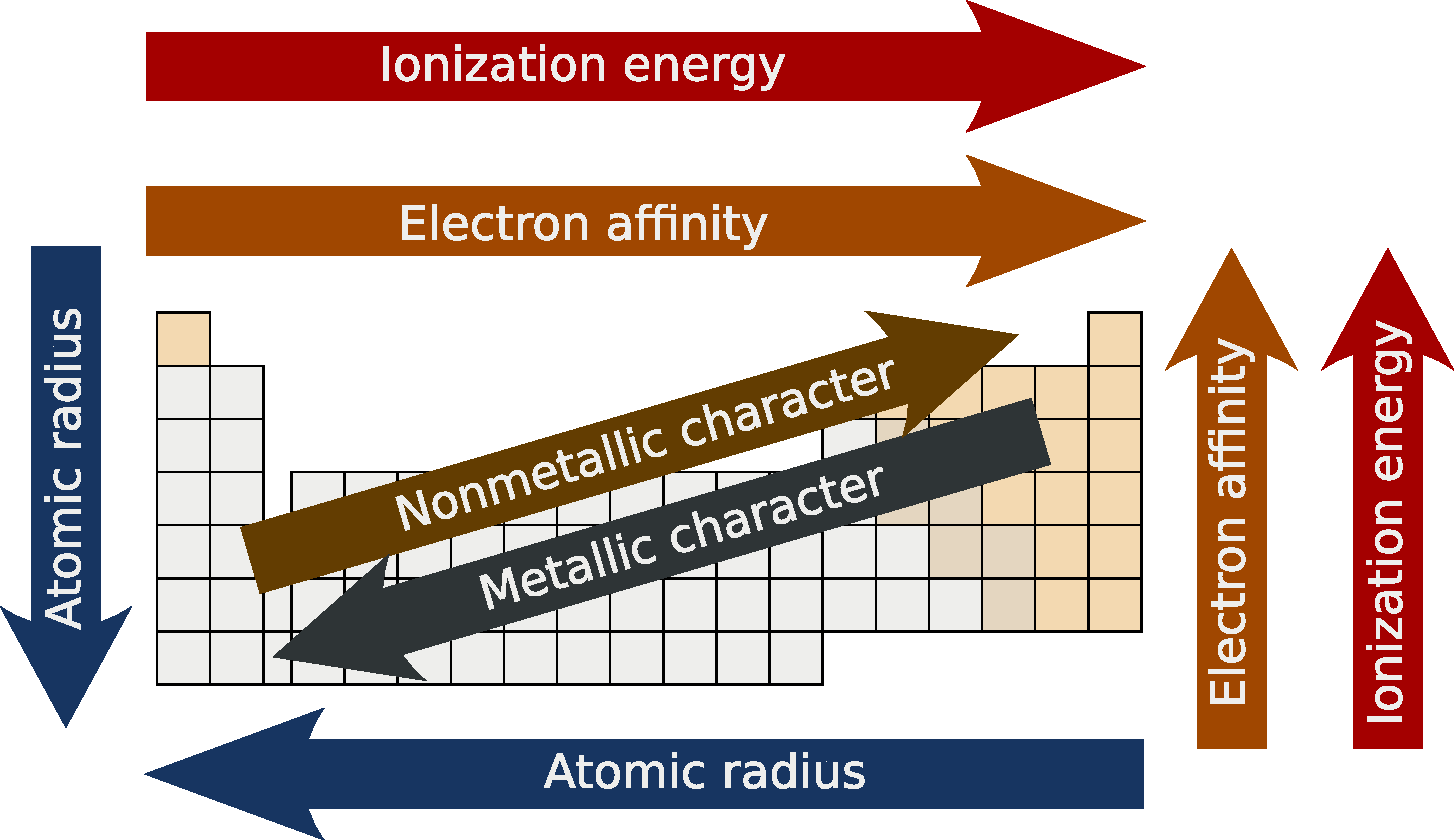
\includegraphics[width=1\linewidth]{src/1_basics/Periodic_trends.pdf}